% Metódy inžinierskej práce

\documentclass[10pt,twoside,slovak,a4paper,twocolumn]{article}

\usepackage[slovak]{babel}
\usepackage[IL2]{fontenc}
\usepackage[utf8]{inputenc}
\usepackage{graphicx}
\usepackage{subcaption}
\usepackage{url}
\usepackage{hyperref}
\usepackage{cite}

\pagestyle{headings}

\title{Stealth Characters Enhanced by Neural Training (SCENT)\thanks{Semestrálny projekt v predmete Metódy inžinierskej práce}}

\author{Omny-1 \and e12dam\\[2pt]
	{\small Slovenská technická univerzita v Bratislave}\\
	{\small Fakulta informatiky a informačných technológií}\\
	{\small \texttt{...@stuba.sk}}
	}

\date{\today}

\begin{document}

\maketitle

\begin{abstract}
Nepriateľské postavy v stealth hrách bývajú často riadené vopred definovanými pravidlami, vďaka čomu je ich správanie ľahko predvídateľné. Projekt SCENT sa zameriava na vytvorenie herných postáv s rozhodovaním založeným na neurónových sieťach, ktoré využívajú iba realisticky dostupné informácie. V 2D bludisku využíva nepriateľ odhadovací modul „nose“ na lokalizáciu hráča pomocou videných a počutých vnemov bez podvádzania v hernom stave.
\end{abstract}

\section{Úvod}
V tradičných stealth hrách sa nepriatelia pohybujú po vopred stanovených trasách a po strate kontaktu s hráčom sa iba presunú na miesto jeho posledného výskytu. Snaha autorov o vytvorenie náročnejšieho protivníka často vedie k tomu, že mu priamo sprístupnia globálnu pozíciu hráča, čo pôsobí neférovo.

Projekt SCENT overuje trénovanie dvoch protichodných agentov v náhodne generovanom 2D bludisku z pohľadu zhora: zlodeja (\textit{Thief}) a príšery (\textit{Beast}). Zlodej má za úlohu nájsť tri predmety a uniknúť východom v časovom limite 90 sekúnd, zatiaľ čo príšera sa ho snaží chytiť. Ani jedna postava na začiatku nepozná umiestnenie predmetov a nepriateľ nikdy nedostáva skutočnú pozíciu zlodeja.

Štruktúra článku je rozdelená nasledovne: v časti~\ref{architektura} predstavujeme architektúru systému a stavový diagram príšery, časť~\ref{metodologia} popisuje tréning pomocou napodobňovania a algoritmu PPO a časť~\ref{zaver} sumarizuje doterajšie výsledky a prínos projektu.

\begin{figure*}[t]
\centering
\fbox{\parbox{0.95\textwidth}{\centering \textbf{SCENT System Overview:} Integrácia simulačného prostredia \textit{MazeEnvironment}, odhadovacieho modulu \textit{NoseEstimator} a politík agentov trénovaných pomocou algoritmu PPO.}}
\caption{Prehľad celého herného systému cez obe kolóny.}
\label{f:prehlad}
\end{figure*}

\section{Architektúra a správanie agentov} \label{architektura}
Na hľadanie zlodeja využíva nepriateľ samostatnú neurónovú sieť nazývanú „nose“. Táto sieť analyzuje, čo nepriateľ videl, počul a zapamätal si, a na základe toho odhaduje pravdepodobnú polohu hráča.

\begin{figure*}[htbp]
  \centering
  \begin{subfigure}[b]{0.48\textwidth}
    \centering
    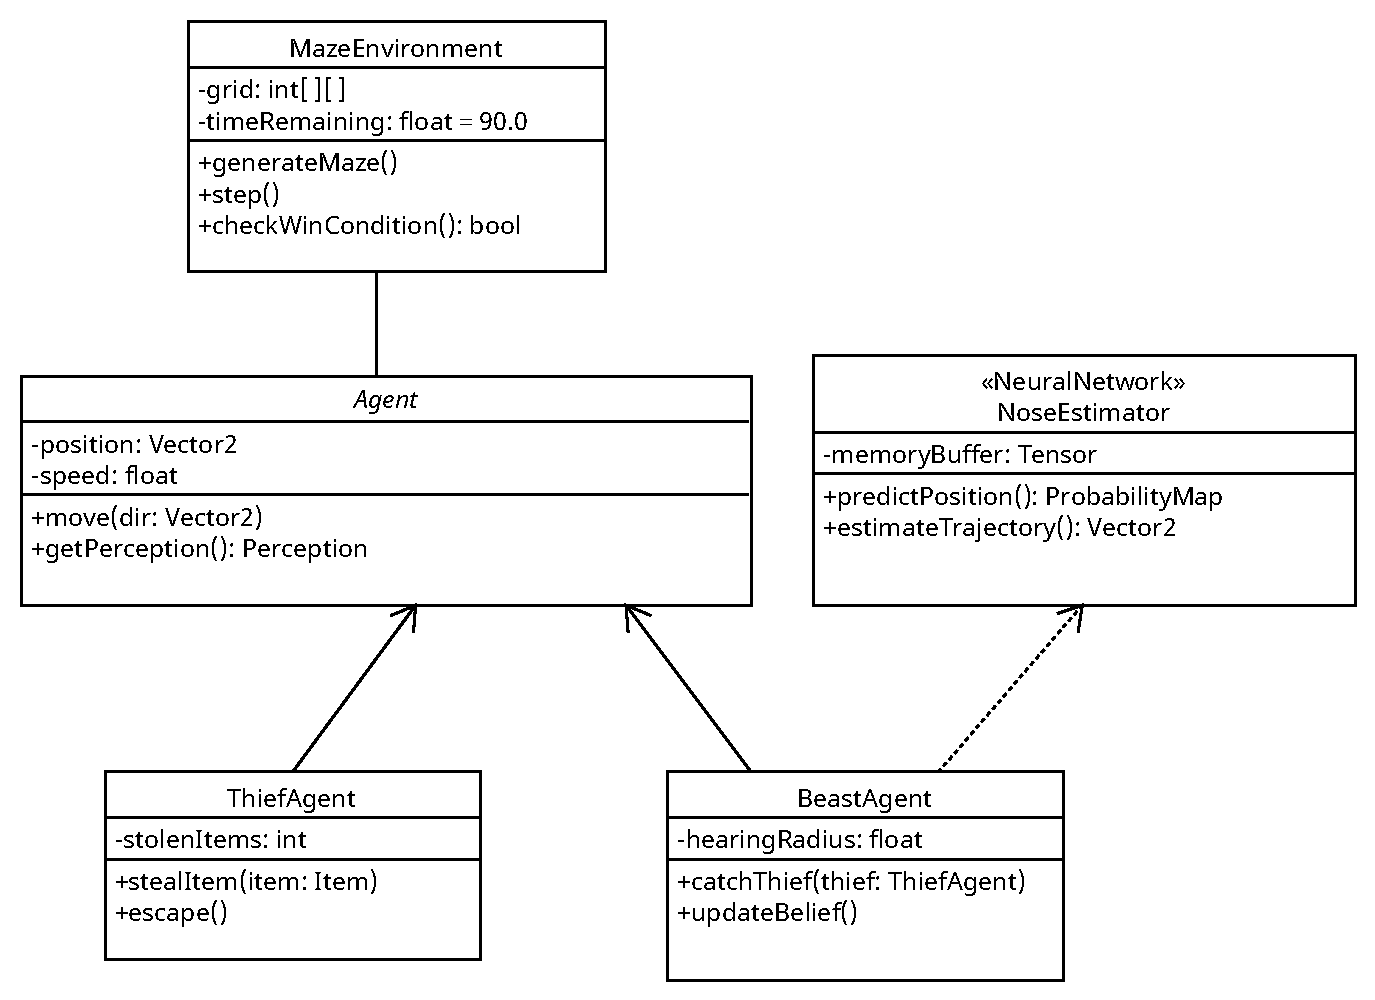
\includegraphics[width=\linewidth]{first_diagram.pdf}
    \caption{Diagram tried systému}
    \label{fig:diag1}
  \end{subfigure}
  \hfill
  \begin{subfigure}[b]{0.48\textwidth}
    \centering
    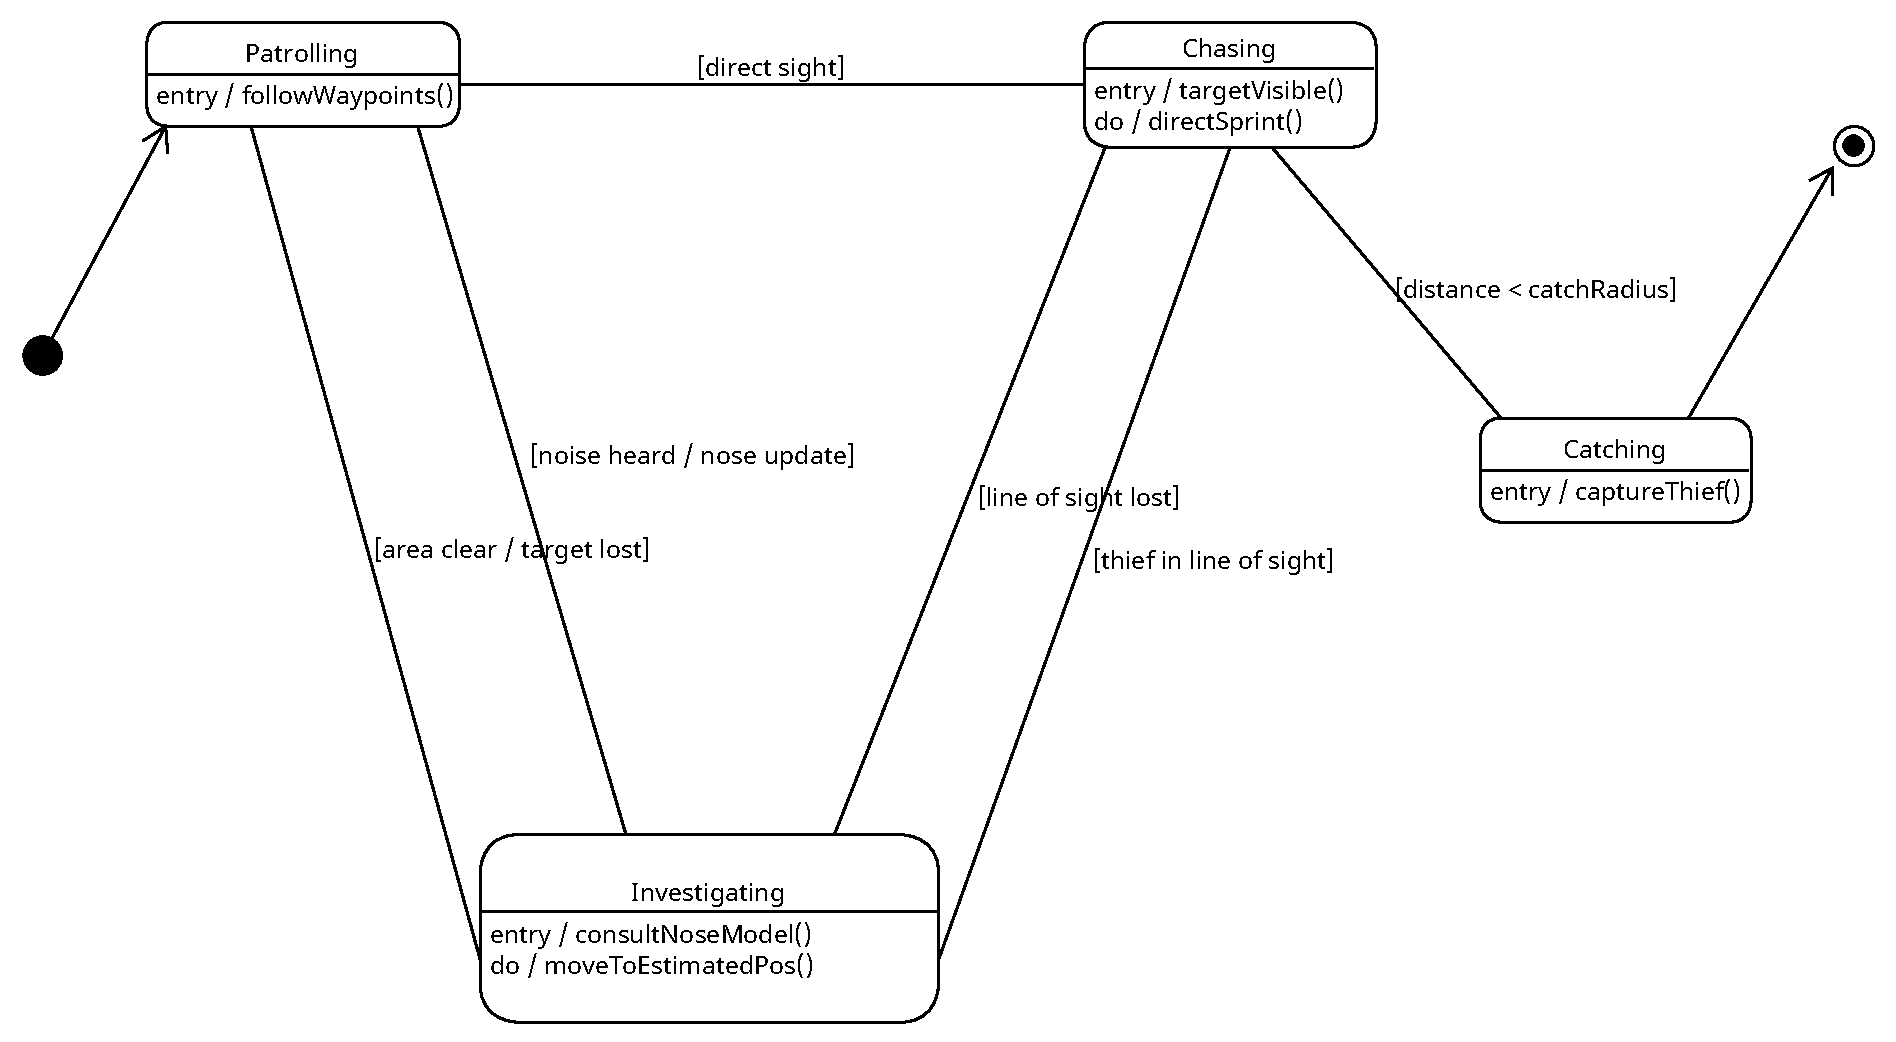
\includegraphics[width=\linewidth]{second_diagram.pdf}
    \caption{Stavový diagram príšery}
    \label{fig:diag2}
  \end{subfigure}
  \caption{UML diagramy systému SCENT}
  \label{fig:dva_diagramy}
\end{figure*}

Na obrázku~\ref{fig:dva_diagramy} sú znázornené vzťahy medzi triedami prostredia a stavový automat rozhodovania príšery, ktorá dynamicky prepína medzi hliadkovaním (\textit{Patrolling}), prešetrovaním zvukov (\textit{Investigating}) a prenasledovaním (\textit{Chasing}).

\section{Metodológia a trénovanie} \label{metodologia}
Každú postavu ovláda vlastná neurónová sieť rozhodujúca o smere pohybu. Agenti sa najprv učia napodobňovaním správania heuristických botov (Behavioral Cloning). Následne prebieha optimalizácia prostredníctvom posilňovaného učenia (Reinforcement Learning) s algoritmom PPO v stovkách tisícov vzájomných hier, kde siete postupne zlepšujú svoje rozhodovanie na základe odmien a trestov.

\section{Vyhodnotenie a záver} \label{zaver}
Prvý prototyp potvrdil významný prínos modulu „nose“: nepriateľ chytil zlodeja v 65\,\% hier s použitím odhadu pozície v porovnaní s iba 31\,\% úspešnosťou bez neho. Projekt sa zameriava aj na testovanie s reálnymi hráčmi s cieľom overiť prirodzenosť a férovosť pohybu nepriateľa. Výsledkom bude hrateľná hra v prehliadači a znovupoužiteľná metodika pre vývoj herných NPC.

\bibliography{literatura}
\bibliographystyle{plain}
\end{document}